\chapter{Cryptography algorithms} % Main chapter title
\label{ch:crypto_algo}

%----------------------------------------------------------------------------------------

\section{Definitions}
We will begin this chapter by giving some useful definitions and theorems.

%-------------------------------------------

\subsection{Finite field (Galois field)}
A \textbf{finite field}, also called a \textbf{Galois field} and usually noted with $F_q$ or $GF(q)$, is a finite set of numbers on a field where multiplication, addition, subtraction and division (excluding division by zero) are defined and satisfy the rules of arithmetic known as the \textit{field axioms}:

\begin{itemize}
    \item associativity of addition and multiplication: $a + (b + c) = (a + b) + c$ and $a \cdot (b \cdot c) = (a \cdot b) \cdot c$;
        
    \item commutativity of addition and multiplication: $a + b = b + a$ and $a \cdot b = b \cdot a$;
    
    \item additive and multiplicative identity: there exist two different elements $0$ and $1$ in $F_q$ such that $a + 0 = a$ and $a \cdot 1 = a$;

    \item additive inverses: for every $a$ in $F_q$, there exists an element in $F_q$, denoted $-a$ and called the \textit{additive inverse} of $a$, such that $a + (-a) = 0$;
    
    \item multiplicative inverses: for every $a \neq 0$ in $F_q$, there exists an element in $F_q$, denoted by $a^{−1}$ or $\frac{1}{a}$ and called the \textit{multiplicative inverse} of $a$, such that $a \cdot a^{−1} = 1$;

    \item distributivity of multiplication over addition: $a \cdot (b+c) = (a \cdot b) + (a \cdot c)$
\end{itemize}

In this set of rules subtraction and division are the inverse operations of addition and multiplication, respectively. In general they are derived from them, but might not be defined as we know them, or it might be possible that they are not defined at all. Also, zero might not be the number zero, but a different element of the field; the same goes for one, the dot and plus: they are just operators. Basically, we have a field of objects that could be anything, and some operations defined on them.

%----------------------

\subsubsection{The Galois field $F_p$}
We can define Galois fields on a number of things; a common field, used in cryptography, is the \textbf{field of all positive numbers from $0$ to $p$}, where $p$ is a \textbf{prime number} or a product of prime numbers.

For each prime number $p$, the \textbf{prime field $F_p$ of order $p$} can be constructed as the integers $modulo\; p$\footnote{Given two positive numbers $a$ and $n$, $a\; modulo\; n$ (abbreviated as $a\; (mod\; n)$) is the remainder of the Euclidean division of $a$ by $n$, where $a$ is the dividend and $n$ is the divisor.}.

\vspace{0.5em}

\emph{Example} Using $p = 7$, a number in $F_7$ is $4$, which can be defined as $11\; (mod\; 7)$, $18\; (mod\; 7)$, etc.

Note that the \textbf{freshman's dream}, as the erroneous equation $(x+y)^n = x^n + y^n$ is sometimes called, is true in $F_p$ for powers of the prime number $p$, because in fields like this we have redefined all operations.

\vspace{0.5em}

\emph{Example} Using $p = 7$, we have:
\begin{center}
$(a + b)^7 = a^7 + 7a^6b + 21a^5b^2 + 35a^4b^3 + 35a^3b^4 + 21a^2b^5 + 7ab^6 + b^7$.
\end{center}

However, since $(7 \cdot x) (mod\; 7) = 0$ \; $\forall x \in F_7$, this means that:
\begin{center}
$(a + b)^7 (mod\; 7) = (a^7 + b^7) (mod\; 7)$.
\end{center}

This is possible because, having redefined all operations, $(a + b)^n (mod\; 7)$ can be rewritten in $F_p$ as:
\begin{center}
$\big((a + b) \cdot (a + b) \cdot ... \cdot (a + b)\big) (mod\; 7) = (a + b) (mod\; 7) \cdot (a + b) (mod\; 7) \cdot ... \cdot (a + b) (mod\; 7)$.
\end{center}

%-------------------------------------------

\subsection{Euler's totient function $\phi(n)$}
\textbf{Euler's totient function $\phi(n)$} counts the \textbf{relatively prime}\footnote{Two integers are \textbf{relatively prime} (or \textbf{coprime}) if there is no integer greater than one that divides them both (that is, their greatest common divisor is 1). Note that they do not have to be both prime (for example, the numbers 8 and 15 are coprime, but neither is prime).} positive integers up to a given integer $n$. In other words, it is the number of integers $k$ in the range $1 \leq k \leq n$ for which the greatest common divisor $gcd(n, k)$ is equal to 1, or how many relative primes exist that are smaller than $n$. The integers $k$ of this form are sometimes referred to as \textit{totatives} of $n$.

\vspace{0.5em}

\emph{Example} The totatives of $n = 9$ are the six numbers 1, 2, 4, 5, 7 and 8. They are all relatively prime to 9, but the other three numbers in this range, 3, 6, and 9 are not, since $gcd(9, 3) = gcd(9, 6) = 3$ and $gcd(9, 9) = 9$. Therefore, $\phi(9) = 6$.

\vspace{0.5em}

\emph{Example} $\phi(1) = 1$ since for $n = 1$ the only integer in the range from 1 to $n$ is 1 itself, and $gcd(1, 1) = 1$.

%----------------------

\subsubsection{Notable facts about $\phi(n)$}
\begin{itemize}
    \item If $p$ is a prime number and $k \geq 1$, then $\phi(p^k) = p^{k-1}(p - 1) = p^k(1 - \frac{1}{p})$.
    \item If $p$ and $q$ are coprime numbers, then $\phi(pq) = \phi(p)\phi(q)$.
    \item If $p$ and $q$ are \textit{both prime} numbers, then $\phi(pq) = (p-1)(q-1)$.
\end{itemize}

%----------------------

\subsubsection{Computing Euler's totient function}
There is no efficient way to calculate the totient function $\phi(x)$, even if we know that $x=pq$ and that $p$ and $q$ are prime numbers.

This happens because even in this case we still need to calculate the divisors of these numbers, and there is no (efficient) algorithm to find them; basically, all we can do is to try dividing our number for all numbers up to it (a brute force method).

Obviously, if we know that $x = pq$ \textit{and} either $p$ or $q$, we can easily find $\phi(x)$ - but this should never be the case in real life applications.

%----------------------

\subsection{Euler's theorem}
\textbf{Euler's theorem} (also known as the \textbf{Fermat–Euler theorem} or \textbf{Euler's totient theorem}) states that if $n$ and $a$ are coprime positive integers, then $a$ raised to the power of the totient of $n$ is equal to $1 (mod\; n)$, or:

\begin{equation}
    a^{\phi(n)} \equiv 1 (mod\; n)
\end{equation}

The definition of a Galois field tells us that the inverse of addition and multiplication \textit{exist}, but not \textit{how} they are defined. Usually they are defined in terms of regular addition and multiplication, but since this is not always possible (because in integer mathematics there is no division as we know it), we use this theorem to calculate the \textbf{multiplicative inverse}, which for a finite field such as a Galois field $F_{\phi(n)}$ is:

\begin{equation}
     a^{\phi(n)} = a \cdot  a^{\phi(n)-1} = a \cdot 1 (mod\; n) = a \;\;\;\;\;\;\;\;\;\; \forall a\neq 0
\end{equation}

%----------------------

\subsubsection{Chinese remainder theorem}
The \textbf{Chinese remainder theorem} states that if we know the remainders of the Euclidean division of an integer $n$ by several integers, then we can determine uniquely the remainder of the division of $n$ by the product of these integers, under the condition that the divisors are pairwise coprime.

We only mention this theorem, as we are not interested in its details. It is important, however, because together with Euler's totient theorem it is used in the \textbf{RSA cryptographic algorithm}.

%----------------------

\subsubsection{Trapdoor function}
A \textbf{trapdoor function} is an invertible function of which if we know its secret, then it is dramatically easy to solve; otherwise, it is next to impossible. In other words, we have the function but we do not know its inverse nor can we calculate it.

Clearly, a trapdoor function is desirable for making a good encryption algorithm, in order to make sure than encryption is easy while decryption is impossible or at least infeasible. This function should also be created using a solid mathematical approach (like definitions and theorems) in order to have proof that it is difficult to solve.

%----------------------------------------------------------------------------------------

\section{RSA algorithm}
The \textbf{RSA algorithm} (Rivest–Shamir–Adleman, from the names of the people who publicly described it in 1977) is a public-key cryptographic algorithm that is widely used for secure data transmission. RSA is a relatively slow algorithm, so it is not commonly used to directly encrypt user data. More often, RSA is used to transmit shared keys for symmetric key cryptography, which are then used for bulk encryption/decryption.

The security of RSA relies on the practical difficulty of factoring the product of two large prime numbers, the \textit{factoring problem}. Breaking RSA encryption is known as the \textit{RSA problem}; whether it is as difficult as the factoring problem is an open question. There are no published methods to defeat the system if a large enough key is used.

\newpage

Given:

\begin{itemize}
    \item $p$, $q$ prime numbers (\textit{private});
    \item $n = p \cdot q$ (\textit{public});
    \item $e$, $d$, coprime\footnote{To ensure that $e$ has a multiplicative inverse.} with $\phi(n)$ and multiplicative inverse $mod\; \phi(n)$, i.e. such that $e \cdot d = 1 (mod\; \phi(n)) = k \cdot \phi(n) + 1$ (\textit{private});
\end{itemize}

then, using Euler's totient function:

\begin{itemize}
    \item[] $m \equiv m^{\phi(n)+1}(mod\; n)$
    \item[] $m \equiv m^{k\cdot\phi(n)+1} (mod\; n) \;\;\;\;\; \forall k \in \mathbb{N}$
\end{itemize}

If we choose $e, d$ such that $d = \frac{k\cdot\phi(n)+1}{e}$, then we have:

\begin{itemize}
    \item[] $m \equiv m^{d \cdot e} (mod\; n)$
\end{itemize}

At this point, called $c = m^e (mod\; n)$ the cyphertext, we get:

\begin{itemize}
    \item[] $c^d (mod\; n) = m^{e^d} (mod\; n) = m^{e^{\frac{k\cdot\phi(n)+1}{e}}} (mod\; n) = m^{k\cdot\phi(n)+1} = m$
\end{itemize}

RSA is an interesting algorithm because even if an attacker knows $n$ and $e$, calculating any of the other numbers (either $\phi(n)$ or $d$) is computationally infeasible: although not impossible, it would take thousands of years even by using the best hardware available, due to the complexity of calculating a \textbf{discrete logarithm} and ultimately of \textbf{factorization}, which is a NP-complete problem.

Note, however, that between 1994 and 1996 a new algorithm was discovered, cutting the computational complexity of factorization by 20\%. Also, quantum computers could compute discrete logarithms in polynomial time.

%----------------------------------------------------------------------------------------

\section{Diffie-Hellman-Merkle algorithm}
The \textbf{Diffie–Hellman-Merkle} (DHM) key exchange is a method of securely exchanging cryptographic keys over a public (non-secure) channel, and was one of the first public-key protocols as conceived by Ralph Merkle, Whitfield Diffie and Martin Hellman.

Published in 1976 by Diffie and Hellman, this is the earliest publicly known work that proposed the idea of a private key and a corresponding public key; even though it is a little old, it is quite interesting and still debated. In 1997 it was revealed that James H. Ellis, Clifford Cocks, and Malcolm J. Williamson of GCHQ (\textit{Government Communications Headquarters}, British signals intelligence agency) had already shown in 1969 how public-key cryptography could be achieved. The question of paternity for this algorithm is largely academic, as the GCHQ paper has been ignored even by the GCHQ itself.

Given:

\begin{itemize}
    \item $p$ a very large prime number (\textit{public});
    \item $\alpha$ a primitive root\footnote{
        A \textbf{primitive root} is a number such that $\alpha (mod\; p)$ has multiplicative order $p-1$, or
            \begin{equation*}
                \alpha (mod\; p) \neq \alpha^2 (mod\; p) \neq \alpha^3 (mod\; p) \neq ... \neq \alpha^{p-1} (mod\; p)
            \end{equation*}
            \begin{equation}
                \alpha^i (mod\; p) \neq \alpha^j (mod\; p) \;\;\;\;\;\;\;\;\;\; \forall i,j \in [1, p-1]
            \end{equation}
        It can be demonstrated that there are $\phi(p-1)$ primitive roots for a prime number.
        }  (\textit{public});
\end{itemize}

the algorithm is as follows:

\begin{enumerate}
    \item A and B choose a secret number, $X_a$ and $X_b$ respectively;
    \item A sends to B $Y_a = \alpha^{X_a} (mod\; p)$;
    \item B sends to A $Y_b = \alpha^{X_b} (mod\; p)$;
    \item A computes $K_a = Y_{b}^{X_a} (mod\; p) = (\alpha^{X_b})^{X_a} (mod\; p)$;
    \item B computes $K_b = Y_{a}^{X_b} (mod\; p) = (\alpha^{X_a})^{X_b} (mod\; p)$;
\end{enumerate}

In the end, $K \equiv K_a \equiv K_b$ is the secret key that only A and B know. It is clear that DHM is similar to RSA, as they both make use of an exponential function of the type $c=m^e$ and need a logarithm (a discrete logarithm) as its inverse function.

This algorithm \textit{must} be paired with an identity verification mechanism, because an \textit{on-path} attacker could easily modify $Y_a$ and $Y_b$. We cannot crack DHM in linear time, unless we have a table of all primitive roots (since the only way to calculate a logarithm is to use tables or successive approximations) - which is is why we need $p$ very large: an inverse table for the logarithm function is possible to create, but if $p$ is large enough it would require too much space, making it infeasible.

%----------------------------------------------------------------------------------------

\section{One-time pad algorithm}
The \textbf{one-time pad} (OTP) is an encryption technique that cannot be cracked, but requires the use of a one-time pre-shared key the same size as, or longer than, the message being sent. In this technique, a plaintext $m$ is paired with a random secret key $k$ (also referred to as a one-time pad), then each bit or character of the plaintext is encrypted by combining it with the corresponding bit or character from the pad using modular addition (an invertible function): cyphertext will be $c=m\oplus k$, while decryption will be $m=c\oplus k$.

The resulting ciphertext will be impossible to decrypt or break if the following four conditions on the key $k$ are met:

\begin{enumerate}
    \item $k$ must be \textbf{truly random}\footnote{Every single bit has exactly a 50\% probability of being either $0$ or $1$.};
    \item $k$ must be at least \textbf{as long as the plaintext};
    \item $k$ must \textbf{never be reused} in whole or in part;
    \item $k$ must be kept \textbf{completely secret}.
\end{enumerate}

The one-time pad has a property termed \textbf{perfect secrecy}; that is, the ciphertext $c$ gives absolutely no additional information about the plaintext. This is because, given a truly random key that is used only once, a ciphertext can be translated into any plaintext of the same length, and all are equally likely. Thus, the a priori probability of a plaintext message $m$ is the same as the a posteriori probability of a plaintext message $m$ given the corresponding ciphertext.

%----------------------

\subsection*{OTP limitations}

The main problem with this algorithm is, of course, getting a perfectly random key $k$. Also, having a key that is as long as the message might be practically impossible.

A solution would be to generate the key with a pseudo-random number generator, and just
exchange the seed of the generator. This might look like a nice idea, but the pseudo-random number generator must really be generating random numbers - so in reality it does not actually work, because it will always have some kind of issue (like correlations between bits, or doubles, or triples, etc.) and, being \textit{pseudo}-random, it is an algorithm, meaning that if one knows the seed, he or she also knows the generated number. The better a pseudo-random generator is, the slower it executes; all of them, however, have at least a problem: their randomness depends entirely on the seeds, which must have certain properties in order to be effective.

%----------------------------------------------------------------------------------------

\section{Confusion and diffusion}
In cryptography, \textbf{confusion} and \textbf{diffusion} are two properties of the operation of a secure cipher identified by Claude Shannon in his 1945 classified report \textit{A Mathematical Theory of Cryptography}. These properties, when present, work to confuse the application of statistics and other methods of cryptanalysis.

These concepts are important in the design of robust hash functions and pseudo-random number generators, where \textbf{decorrelation} of the generated values is of paramount importance; basically, they should be enforced in algorithms in order to \textbf{prevent statistical cryptanalysis}.

These properties, however, are not mandatory for an algorithm to be safe. As an example, the one-time pad algorithm, which generates a ciphertext statistically independent of the plaintext, relies \textit{not} on either confusion, nor diffusion (this one because every bit of plaintext depends on a single bit of the key). This is true for all stream ciphers, because they are immune by definition to statistical cryptanalysis. Note that it might be argued that OTP does make use of confusion as the secret is not really the key $k$, which has the same length as $m$ and $c$, but the seed which generated it assuming that $k$ has been created using a pseudo-random number generator).

%----------------------

\subsection*{Confusion}
\textbf{Confusion} means that each binary digit (bit) of the ciphertext should depend on several parts of the key, obscuring the connections between the two. This property hides the relationship between the ciphertext and the key.

Confusion also makes it difficult to find the key from the ciphertext, and if a single bit in a key is changed, the calculation of the values of most or all of the bits in the ciphertext will be affected; it basically increases the \textbf{ambiguity} of ciphertext.

%----------------------

\subsection*{Diffusion}
\textbf{Diffusion} means that if we change a single bit of the plaintext, then (statistically) half of the bits in the ciphertext should change, and similarly, if we change one bit of the ciphertext, then approximately one half of the plaintext bits should change. Since a bit can have only two states, when they are all re-evaluated and changed from one seemingly random position to another, half of the bits will have changed state. In other words, the idea of diffusion is to \textbf{hide the relationship} between the ciphertext and the plain text.

%----------------------------------------------------------------------------------------

\section{Substitution algorithms}
\textbf{Substitution} algorithms are part of the so-called \textbf{Substitution-Permutation Networks} (SPNs), proposed by Shannon for the creation of robust and practical ciphers, such as the Feistel cipher. The one-time pad also is a special case of substitution algorithm.

Let us consider the case of block ciphers\footnote{A \textbf{block cipher} is a deterministic algorithm operating on fixed-length groups of bits, called \textit{blocks}.} on $n$ bits. In the most general case, for a fixed key $k$, such a cipher simply consists of an injective function $f$ from blocks of $n$ bits to blocks of $n$ bits or, in other words, a (static) map that changes the bits of a message:

\begin{equation*}
    f: \{ 0, 1\} \rightarrow \{ 0, 1\}^n
\end{equation*}

\emph{Example} Consider the following function for $n=2$ (2-bit map), where $f$ is a permutation of $\{0, 1\}^2.$:

\begin{center} % Centered list
$00 \rightarrow 01$\\
$01 \rightarrow 11$\\
$10 \rightarrow 00$\\
$11 \rightarrow 10$\\
\end{center}

\vspace{0.5em}

In the most general case, the number of possible transformations is equal to the possible permutations of the $2^n$ blocks, or $n^{n!}$. If we use small blocks, e.g. with $n=4$ or $n=5$, we get a classic monoalphabetic substitution cipher\footnote{In such a cipher, any character of plaintext from a given fixed set of characters is substituted by some other character from the same set.}.

Clearly, these ciphers are subscetible to \textbf{statistical cryptanalysis} attacks, because they do not have diffusion. In order to mitigate this risk we could use larger maps, but this is not feasible because the keys would have too many bits to be actually used in practice.

\vspace{0.5em}

\emph{Example} Given a 64-bit map ($n=64$), which is reasonably secure, the key would be represented by the permutation itself, which would be coded as $n\cdot 2^n = 64 \cdot 2^{64} \approx 10^{21}$. This is an impossible number of bits for a computer to handle.

%----------------------------------------------------------------------------------------

\section{Feistel cipher}
A \textbf{Feistel cipher} is a symmetric structure used in the construction of block ciphers, named after Horst Feistel who did pioneering research while working for IBM.

In a Feistel cipher, encryption and decryption are very similar operations, and both consist of iteratively running a function called a \textit{round function}\footnote{A \textbf{round function} is a function which takes two inputs, a data block and a subkey, and returns one output the same size as the data block.} a fixed number of times; the algorithm works as follows (also see fig. \ref{fig:feistel}):

\begin{enumerate}
    \item plaintext is divided in two parts $L_0$ and $R_0$, each of $w$ bits;
    \item $L_0$ and $R_0$ both go through $n$ rounds which have the same structure (plaintext is modified by a function $F$ which performs \textit{diffusion}) but use $n$ subkeys $K_1, ..., K_n$ generated from the main key $K$ such that $K_i \neq K_j \;\;\; \forall i, j \in [1, n], i \neq j$, and $K_i \neq K \;\;\; \forall \in [1, n]$;
    \item the two parts of plaintext exit the last round as $L_n$ and $R_n$ and go through a last step which swaps them (creating $L_{n+1}$ and $R_{n+1}$) to perform \textit{confusion}.
\end{enumerate}

The function $F$ is a cryptographically secure pseudo-random permutation function, where $K_i$ is the seed. This scheme is (more or less) used by all symmetric encryption algorithms.

An important advantage of Feistel ciphers is that the entire operation is guaranteed to be invertible (that is, encrypted data can be decrypted), even if the round function is not itself invertible. The round function can be thus made arbitrarily complicated, since it does not need to be designed to be invertible. Furthermore, the encryption and decryption operations are very similar, even identical in some cases; therefore, the size of the code or circuitry required to implement such a cipher is nearly halved: this cipher is easily translated into hardware.

\begin{figure}[H]
    \centering
    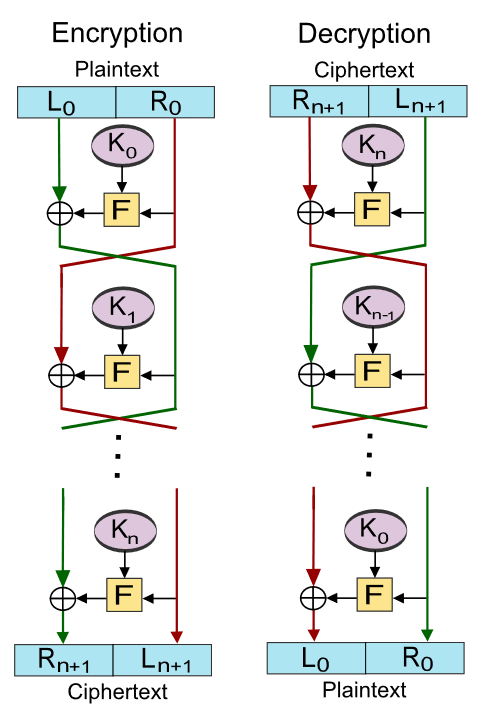
\includegraphics[scale=0.5]{img/feistel.png}
    \decoRule
    \caption{Feistel cipher encryption and decryption.}
    \label{fig:feistel}
\end{figure}

%----------------------------------------------------------------------------------------

\section{Elliptic curve cryptography}
\textbf{Elliptic curve cryptography} (ECC) is one of the most powerful but least understood types of cryptography in wide use today\footnote{Sullivan Nick, \textit{A (relatively easy to understand) primer on elliptic curve cryptography}, Ars Technica}. An increasing number of websites make extensive use of ECC to secure everything, from customers' HTTPS connections to how they pass data between data centers. It has fantastic pros and fantastic cons, but since we still do not know when and if there will be some way to invert it, we should not use it to encrypt very important stuff.

After the introduction of the RSA and Diffie-Hellman algorithms, researchers explored additional mathematics-based cryptographic solutions looking for other algorithms beyond factoring that would serve as good \textbf{trapdoor functions}. In 1985, cryptographic algorithms were proposed based on an esoteric branch of mathematics called \textit{elliptic curves}.

\begin{figure}[H]
    \centering
    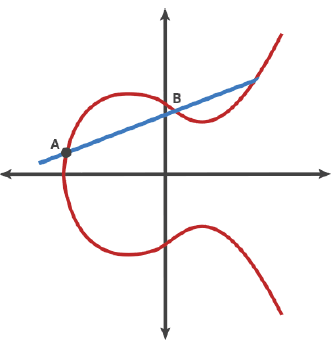
\includegraphics[scale=1]{img/elliptic.png}
    \decoRule
    \caption{An elliptic curve.}
    \label{fig:elliptic}
\end{figure}

An elliptic curve is a mathematical function of the form y$^2 = x^3 + ax + b$, as shown in fig. \ref{fig:elliptic}. It has two interesting properties:

\begin{itemize}
    \item it is symmetric with respect to the $x$-axis;
    \item any non-vertical line will intersect the curve in at most three places.
\end{itemize}

Let us imagine this curve as the setting for a bizarre game of billiards. Take any two points on the curve and draw a line through them; the line will intersect the curve at exactly one more place. In this game of billiards, we take a ball at point $A$ and shoot it toward point $B$. When it hits the curve, the ball bounces either straight up (if it is below the $x$-axis) or straight down (if it is above the $x$-axis) to the other side of the curve.

We can call this billiards move on two points a \textbf{dot function}. Any two points on a curve can be \textit{dotted} together to get a new point:

\begin{equation}
    A\; dot\; B = C
\end{equation}

We can also chain moves together to \textit{dot} a point with itself over and over:

\begin{center}
    $A\; dot\; A = B$ (this is the line tangent to the elliptic curve)\\
    $A\; dot\; B = C$ (also, $A\; dot\; B = B\; dot\; A$)\\
    $A\; dot\; C = D$
\end{center}

Basically, if we have two points and an initial point \textit{dotted} with itself $n$ times to arrive at a final point, finding out $n$ when we only know the final point and the first point is hard. To continue our bizarro billiards metaphor, imagine that one person plays our game alone in a room for a random period of time. It is easy for him or her to hit the ball over and over following the rules described above. If someone walks into the room later and sees where the ball has ended up, even if they know all the rules of the game and where the ball started, they cannot determine the number of times the ball was struck to get there without running through the whole game again until the ball gets to the same point. Easy to do, hard to undo: this is the basis for a very good trapdoor function.

Every couple of points $A$ and $B$ have a result $C$, because the elliptic curve is defined from a point called a \textbf{null point} and goes up to \textbf{infinity}, so on the $x$-axis from the null point (negative) to infinity (positive) we have every single $x$ covered.

Let us restrict ourselves to numbers in a fixed range like in RSA, meaning that rather than allowing any value for the points on the curve, we restrict ourselves to whole numbers in a fixed range. When computing the formula for the elliptic curve $y^2 = x^3 + ax + b$, we use the same trick of rolling over numbers when we hit the maximum. If we pick the maximum to be a prime number, the elliptic curve is called a \textbf{prime curve} and has excellent cryptographic properties.

\begin{figure}[H]
    \centering
    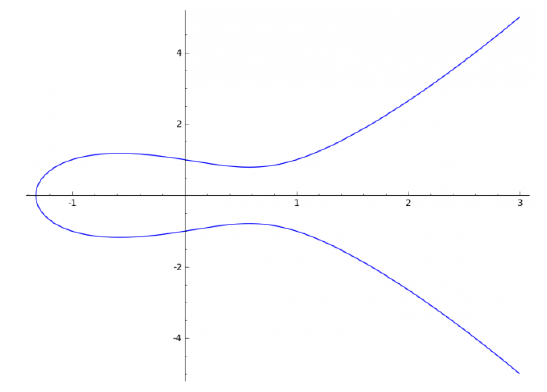
\includegraphics[scale=1]{img/elliptic2.png}
    \decoRule
    \caption{The curve $y^2 = x^3 - x + 1$ plotted for all numbers.}
    \label{fig:elliptic2}
\end{figure}

Figure \ref{fig:elliptic3} hardly looks like a curve in the traditional sense, but it is. It is like the original curve was wrapped around at the edges and only the parts of the curve that hit whole number coordinates are colored in, and we can even still see the horizontal symmetry.

In fact, we can still play the billiards game on this curve and dot points together. The equation for a line on the curve still has the same properties. Moreover, the dot operation can be efficiently computed: we can visualize the line between two points as a line that wraps around at the borders until it hits a point. It is like in our bizarro billiards game, when a ball hits the edge of the board (the max), then is magically transported to the opposite side of the table and continues on its path until reaching a point.

With this new curve representation, we can take messages and represent them as points on the curve. We could imagine taking a message and setting it as the $x$ coordinate and solving for $y$ to get a point on the curve. It is slightly more complicated than this in practice, but that is the general idea.

\begin{figure}[H]
    \centering
    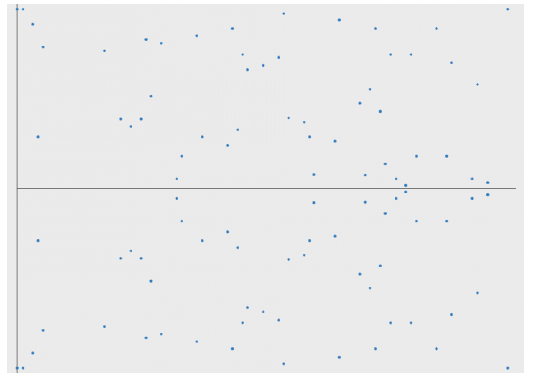
\includegraphics[scale=1]{img/elliptic3.png}
    \decoRule
    \caption{Plot of the same curve as \ref{fig:elliptic2} with only the whole number points represented, with a maximum of $97$.}
    \label{fig:elliptic3}
\end{figure}

An elliptic curve cryptosystem can be defined by picking a prime number as a maximum, a curve equation, and a public point on the curve. A private key is a number $priv$, and a public key is the public point \textit{dotted} with itself $priv$ times. Computing the private key from the public key in this kind of cryptosystem is called the \textbf{elliptic curve discrete logarithm function}. This turns out to be the trapdoor function we were looking for.

Basically, given a seed point $A$, we calculate $A\; dot\; A$ $n$ times: $A\; dot\; A$ will intersect another point $B$. If we do it again we will get another point, and so on. The thing is that if we know the starting point and how many times we elevated $A$ to itself (we did the dot function), calculating the endpoint is very easy, but if we only know the starting point and the endpoint, calculating how many times we did the dot function becomes dramatically harder (basically we will have to try doing it $n$ times).

%-------------------------------------------

\subsection*{Pros of elliptic functions}
The elliptic curve has been proposed by two mathematicians who were working for the NSA. It has been shown that is extremely hard to reverse-engineer, and that security is reached with less bytes in the key with respect to normal algorithms. Usually the shorter the key means the weaker is the algorithm; however, the elliptic curve was demonstrated that it is as strong as other algorithms with a shorter key, which is an extremely nice property: we can save bits and bytes in protocol exchanges and, depending on the algorithm, also be faster.

%-------------------------------------------

\subsection*{Cons of elliptic functions}
The problem that has been spotted almost immediately within the elliptic curve function was that there was no mathematical proof that the problem of inverting an elliptic curve was not treatable. We do not know if there is a way to invert the function; the inventors might have it but did not disclose it. Also, if we choose poorly $A$ and $B$ there might be a clever way to invert the algorithm.

In general, we must always make sure that the algorithms we use are top-notch; we must never use the new ones, which might not have been tested extensively and might suffer from unknown vulnerabilities, but instead we need the older, stronger ones, about which we know many properties.

%----------------------------------------------------------------------------------------

\section{Side-channel attacks}
A side-channel attack, also simply called a \textbf{side attack}, is any attack based on information gained from the \textit{implementation} of a computer system, rather than weaknesses in the implemented algorithm itself (e.g. cryptanalysis and software bugs).

General classes of side attacks include:

\begin{itemize}
    \item \textbf{timing attacks}: the attacker attempts to compromise a cryptosystem by analyzing the time taken to execute cryptographic algorithms. Since every logical operation in a computer takes time to execute, and the time can differ based on the input, with precise measurements of the time for each operation, an attacker can work backwards to the input;
    \item \textbf{heat and power monitoring attack}: the attacker studies the heat generation and/or power consumption of a cryptographic hardware device; by measuring these basic physical properties of a system, it is possible to learn a small amount of information about the data being manipulated;
    \item \textbf{random number generator attack}: the attacker subverts or exploits weaknesses within the process of random number generation. From a hardware point of view, this can be done by trying to either capture radio-frequency emissions from the computer (obtaining hard drive interrupt times from motor noise, for example), or to feed controlled signals into a supposedly random source (such as feeding a strong, known signal into a sound card).
\end{itemize}

In all cases, the underlying principle is that physical effects caused by the operation of a cryptosystem (on the side) can provide useful extra information about secrets in the system like, for example, the cryptographic key, partial state information, full or partial plaintexts and so forth.

The very basic point of all this is that we need to make sure that our algorithm performs either in the same way for any input, or in a random way for any input.